\section{Introduction}
\label{intro}

\begin{figure}[h] \hspace*{0cm} 
\begin{center}
	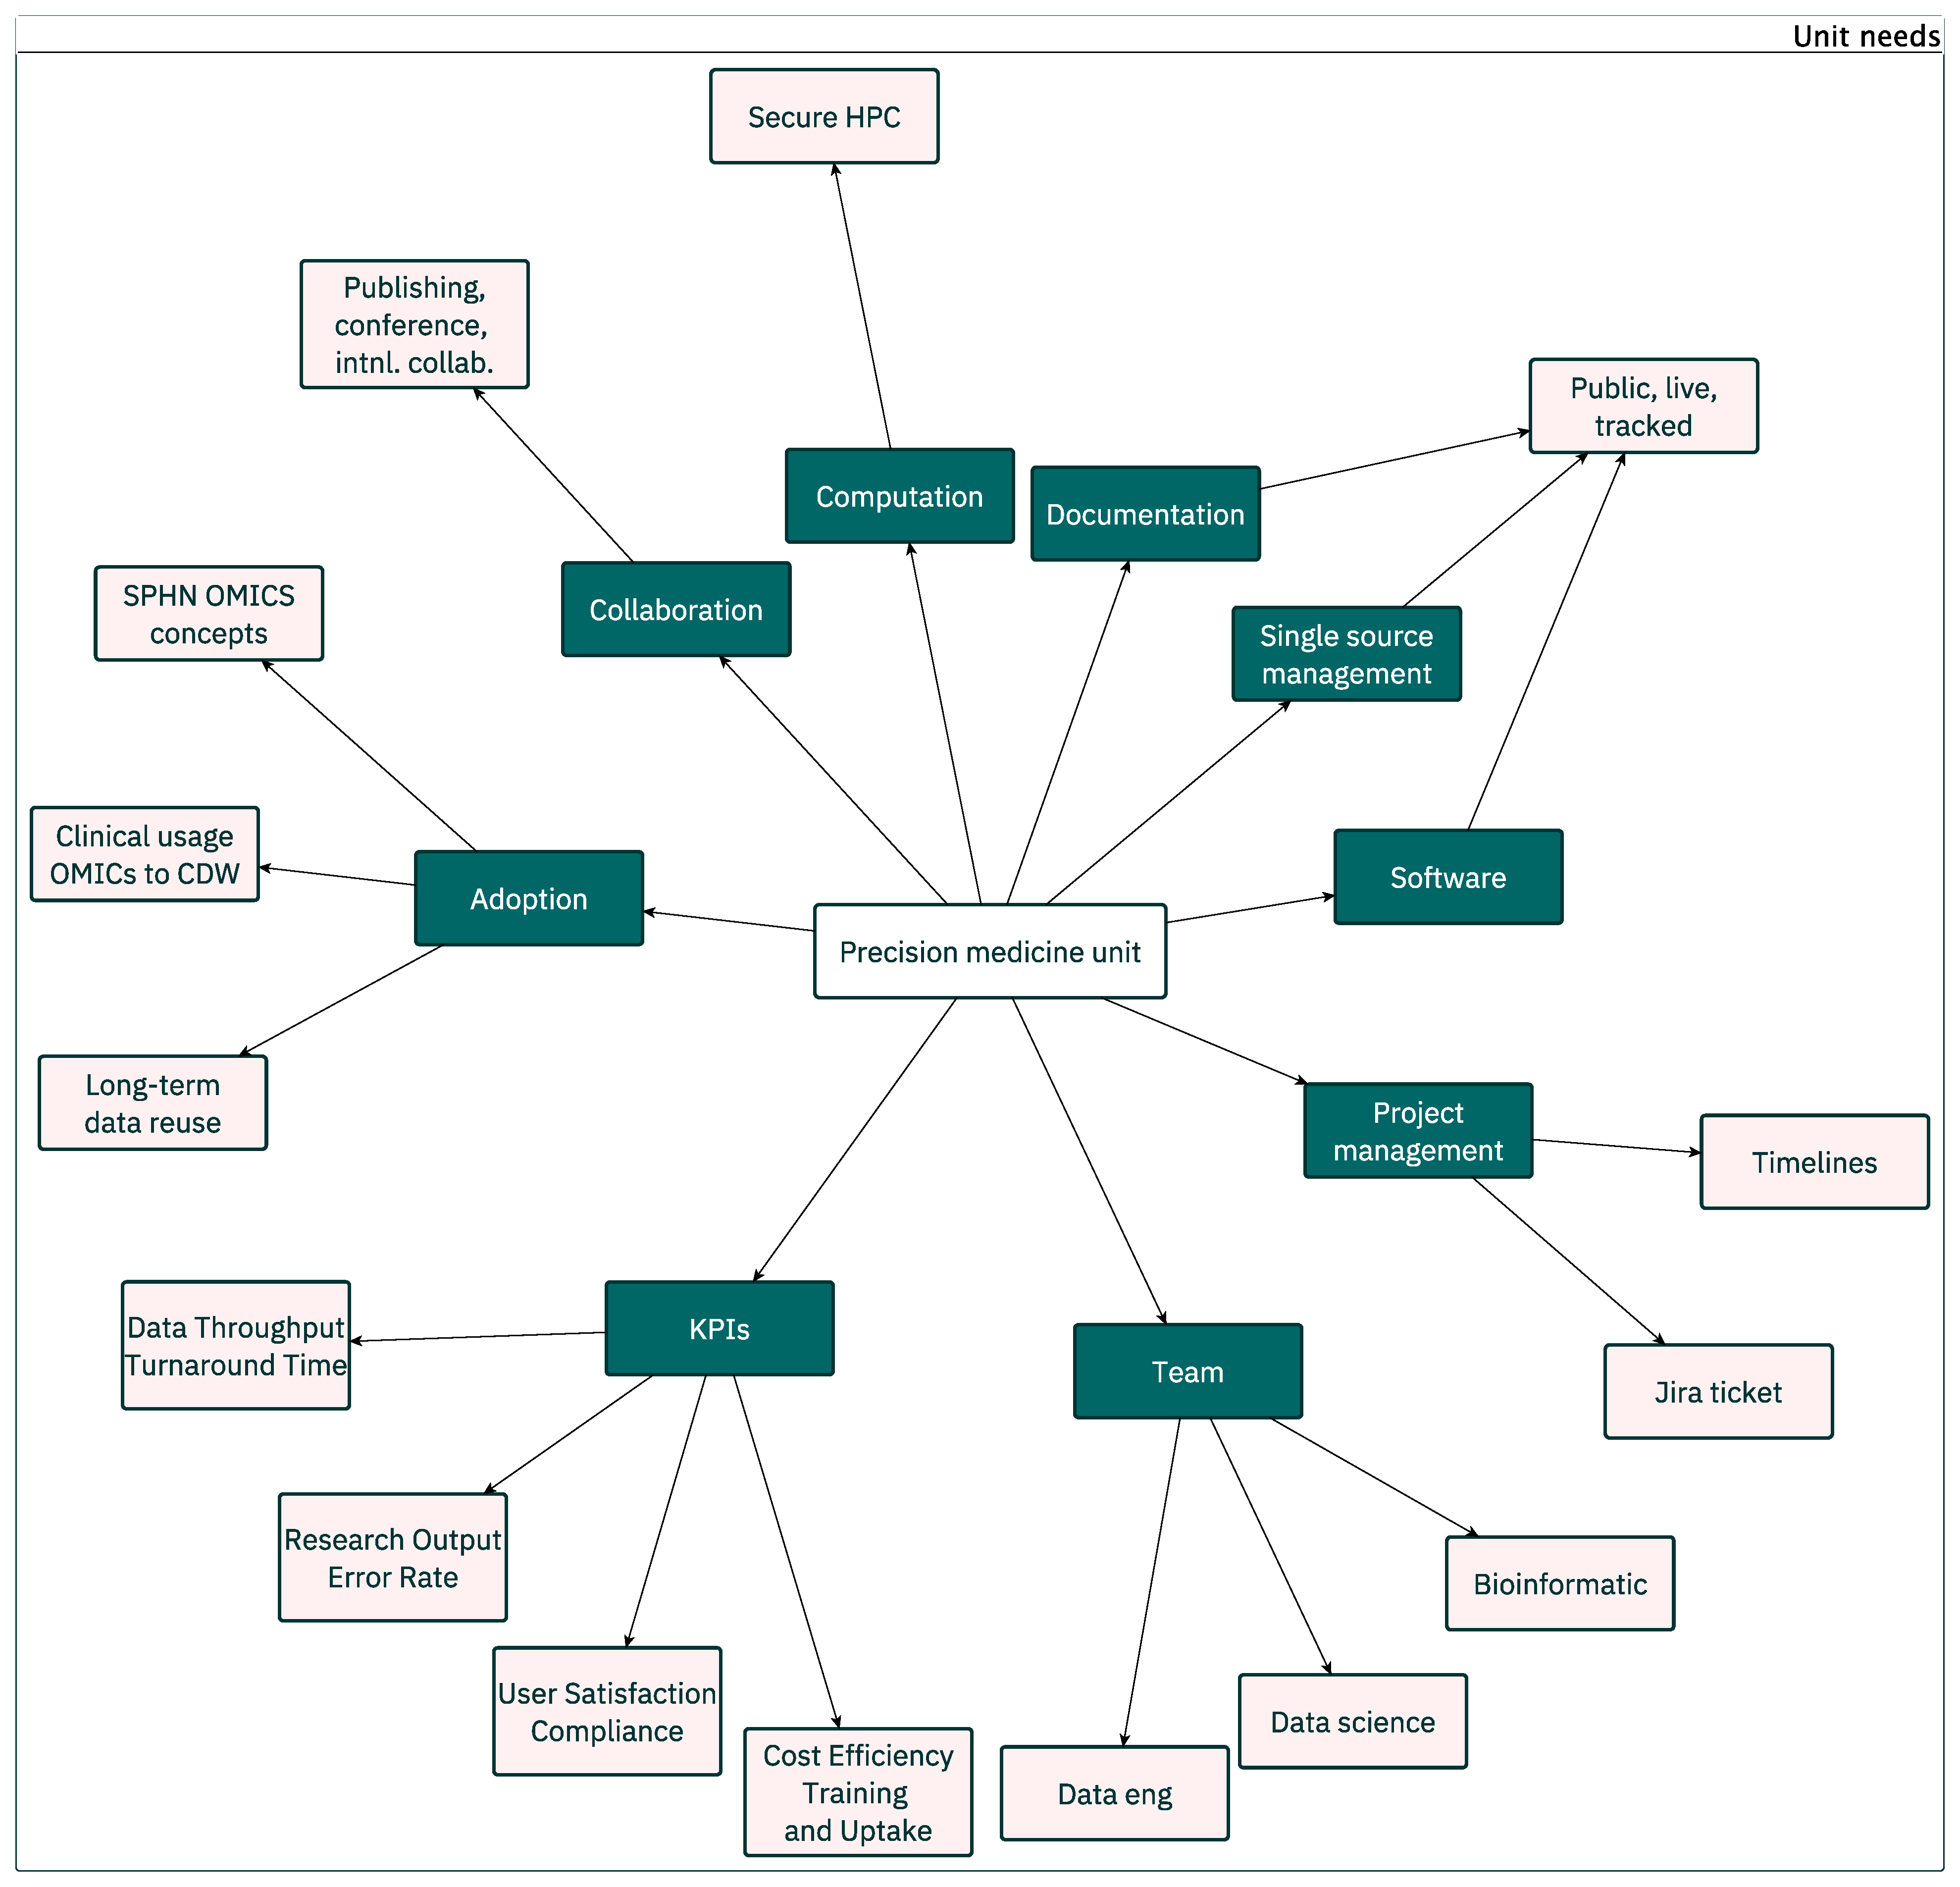
\includegraphics[width=0.48\textwidth]{precision_med_unit_management}
	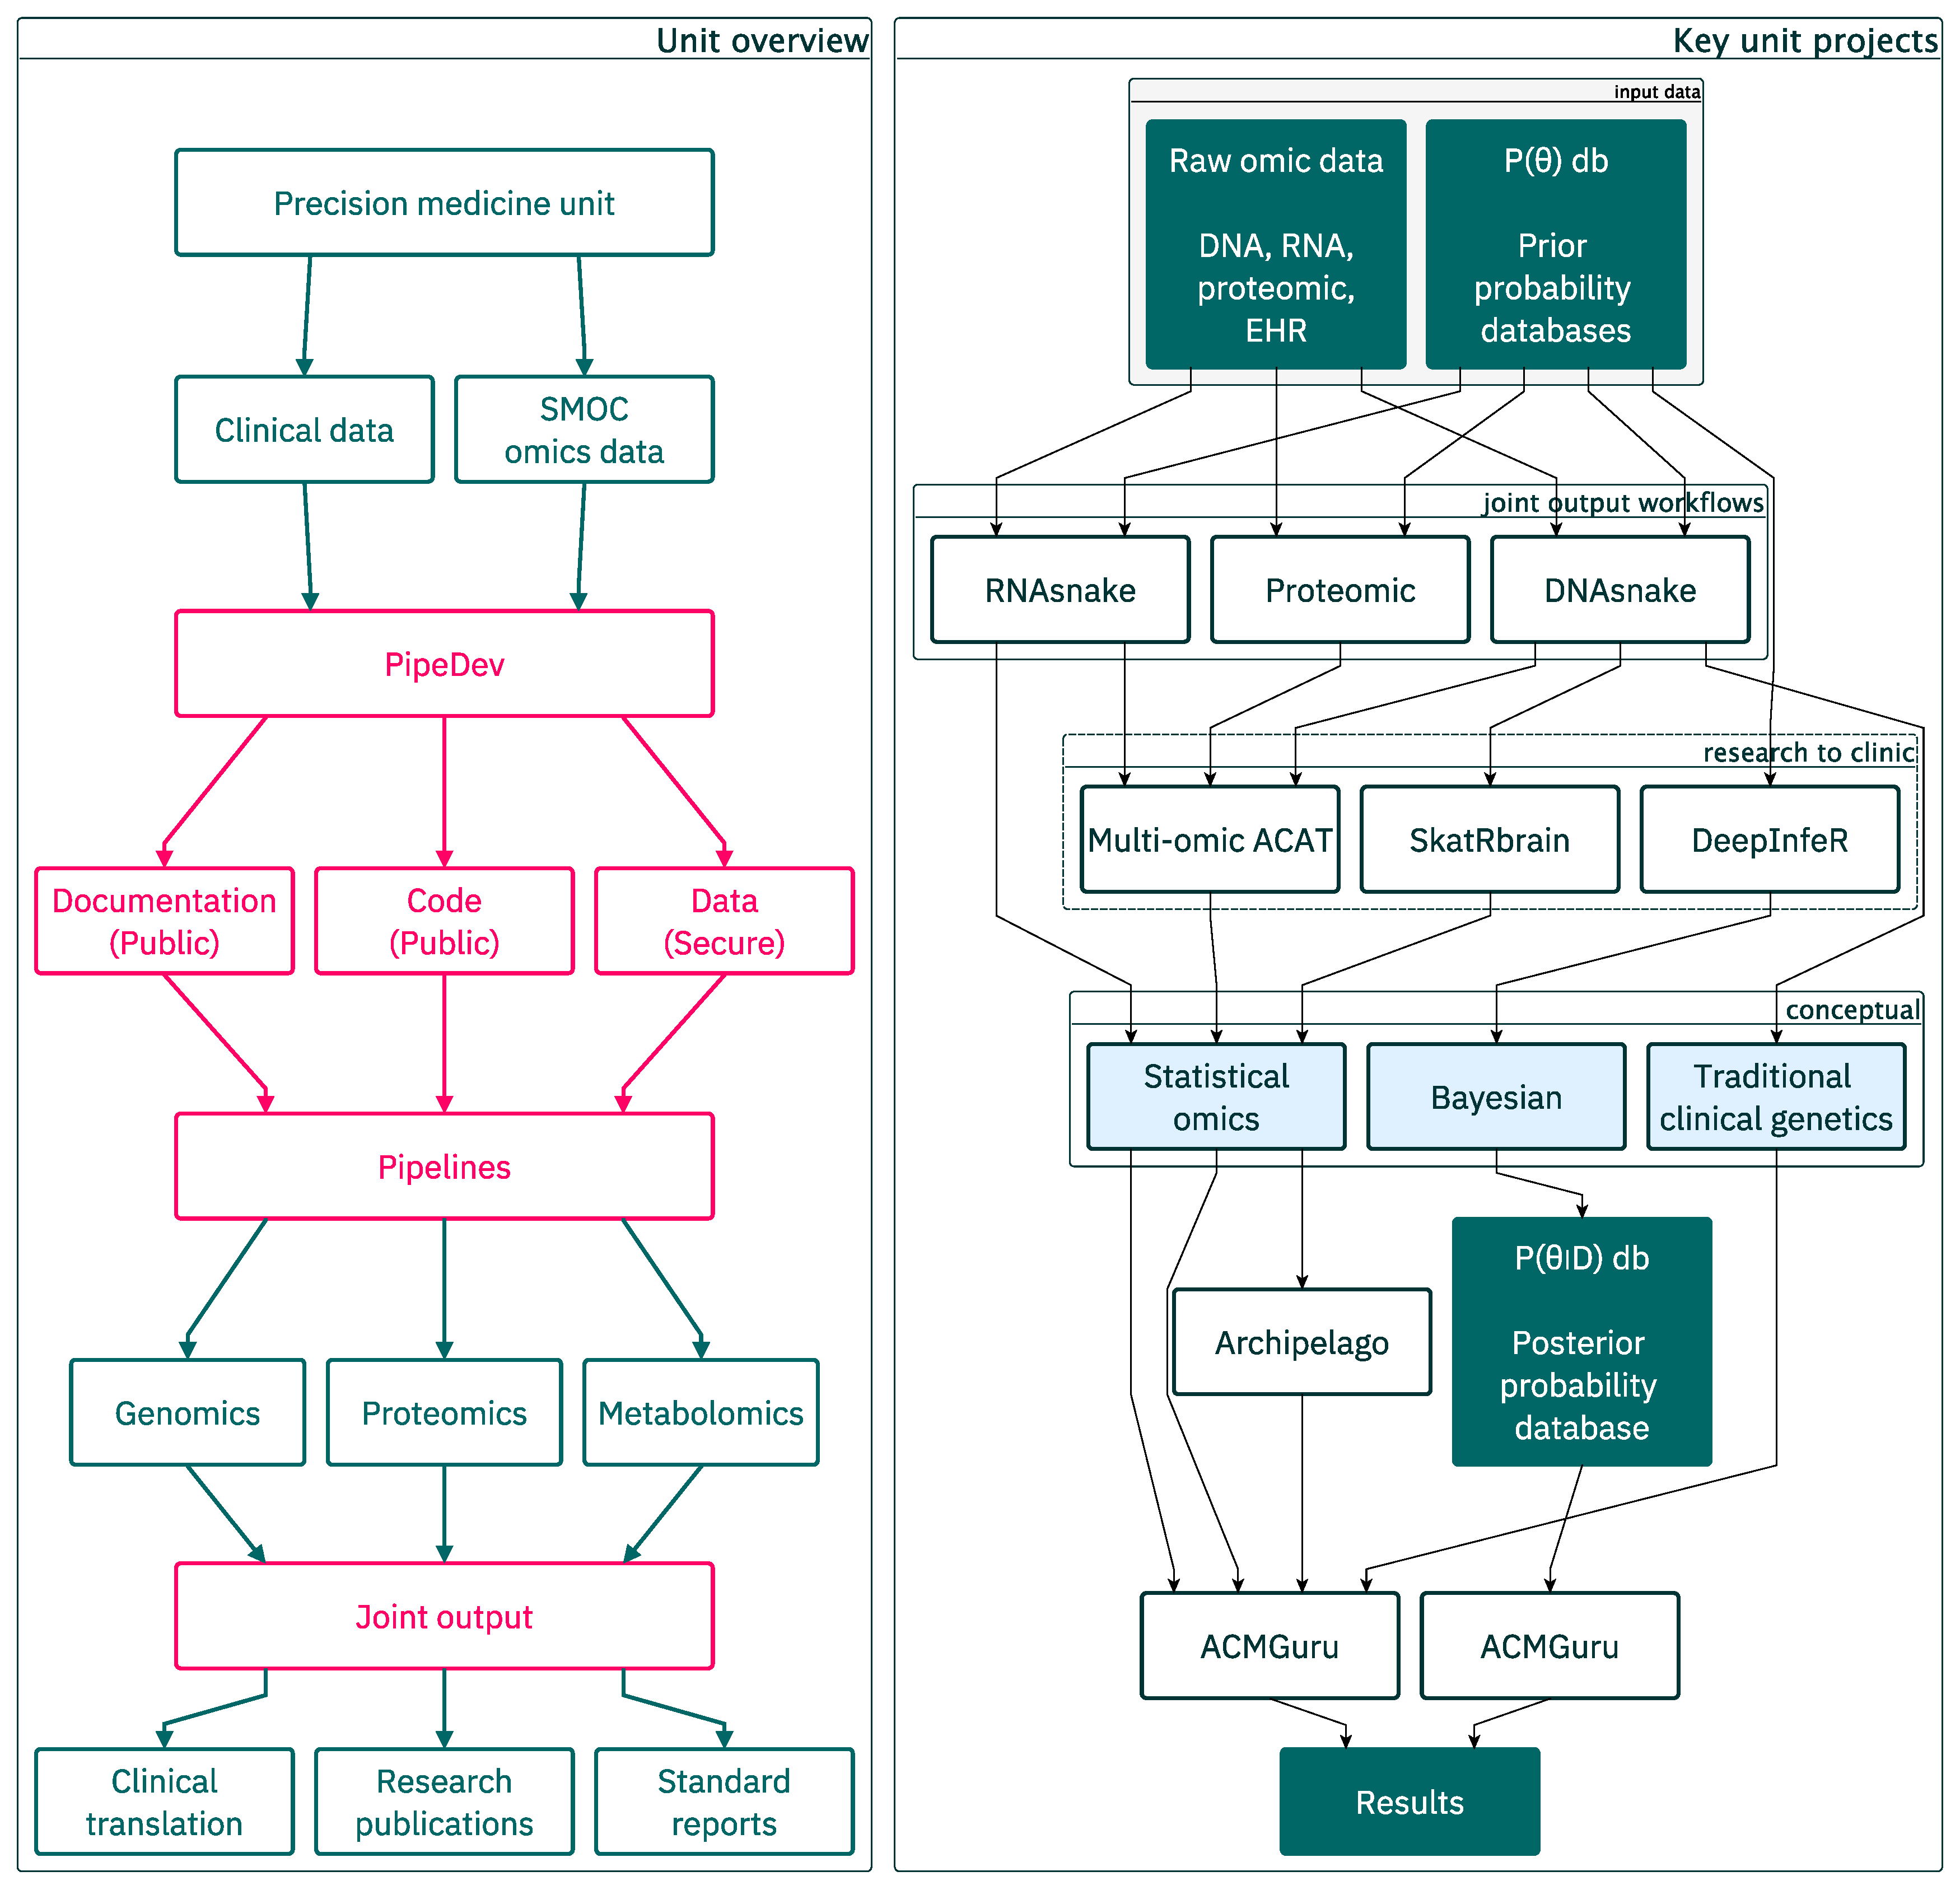
\includegraphics[width=0.48\textwidth]{precision_med_overview}
	\caption{\pmu overview. The unit needs illustrate the management philosophy for minimal disruption for technical progress. The unit overview illustrates the main flow of information to key products. Key unit products illustrate the flow of information, with technical hurdles avoided using the principles of single-source management and shared open development.}
	\label{fig:overview}
\end{center}
\end{figure}

The \pmu is ready to update our paediatric healthcare by serving an array of advanced capabilities in multi-omics, pioneering research methodologies, purpose-built infrastructure, and rigorous data analysis techniques. 
Our approach sets a new benchmark for personalised treatment, employing cutting-edge omics services to provide tailored healthcare for the clinic and 
enrich basic science at \kispi. An overview of our unit is shown in 
\textbf{figure \ref{fig:overview}}.

Traditionally, medical practices have predominantly adhered to a standard approach, tailoring disease prevention and treatment strategies based on the average response anticipated from a general population. 
This conventional method has proven effective for certain patients and conditions, but often falls short when individual variances in genetics, environment, and lifestyle are significant factors influencing health outcomes. 
Precision medicine emerges as a revolutionary paradigm, diverging from the one-size-fits-all approach to embrace these individual differences. 
This innovative medical strategy integrates detailed layers of genomic, environmental, and lifestyle data to tailor personalized healthcare solutions. 
The evolution of precision medicine has been markedly propelled by significant advances in biomedical research, affecting millions worldwide. It aims not only to refine disease treatment and prevention but also promises enhanced outcomes by aligning more closely with each person's unique biological makeup. This approach has profound implications across various domains of healthcare, including oncology, pharmacogenomics, and the management of rare diseases, setting a new standard in personalized healthcare.
Our partners are implementing precision medicine approaches at
the 
\href{https://www.precisionmed.ch/en/}{Swiss Institute of Bioinformatics (SIB)},
\href{https://theloopzurich.ch/en/}{The LOOP Zurich},
\href{https://www.chuv.ch/en/bdsc/research/our-groups/precision-medicine}{CHUV}, 
and all  private industry leaders such as 
\href{https://www.roche.com/about/strategy/personalised-healthcare}{Roche},
\href{https://www.gene.com/topics/personalized-healthcare}{Genentech},
and \href{https://www.pfizer.com/science/innovation/precision-medicine}{Pfizer}.

There have also been many failed promises where precision medicine did not deliver.
However, these failures are typically due to the logistical difficulties of creating an efficient system.
This is not due to inherent problems with the technology. 
Success has been demonstrated by a number of examples in the UK, US, and UAE, which resulted from careful planning and development.

The \pmu at \kispi can be ready to collaborate closely with the Health 2030 Genome Center, part of the Swiss Multi-Omics Center (SMOC) (\url{http://smoc.ethz.ch}), to harness state-of-the-art genomic services. 
This partnership underpins our cutting-edge approach in pediatric healthcare, enabling us to deliver personalised treatment strategies through comprehensive multi-omic data analysis.
As a collaborative effort among major Swiss universities and university hospitals, including UNIBE, Inselspital, UNIL, CHUV, UNIGE, HUG, and EPFL, the center exemplifies a comprehensive approach to personalized health care and genomic research.
SMOC integrates expertise across genomics, transcriptomics, proteomics, and metabolomics. This integrated multi-omic analysis is essential for the thorough exploration and understanding of clinical specimens. Accredited under ISO 15189, the center ensures the highest standards in sequencing and data analysis, leveraging state-of-the-art technologies such as the Illumina Novaseq6000 platforms and TruSeq DNA PCR-Free library preparation.


We will employ essential services such as:
\begin{itemize}
    \item Clinical-grade whole genome sequencing (WGS)
    \item Clinical-grade whole exome sequencing (WES)
    \item Clinical-grade RNA sequencing (RNA-seq)
    \item Fast turnaround time for clinical-grade WGS, WES, and RNA-seq
    \item Low-coverage WGS with variant imputation
    \item Viral pathogen WGS
    \item Microbiome WGS
\end{itemize}

Our subsequent analysis  occurs at the cutting edge of technology, employing the most reliable reference genomes based on GRCh38 and adhering to stringent guidelines for handling sensitive clinical data, as outlined by the SPHN/BioMedIT network on the sciCORE platform (\url{https://sphn.ch/network/projects/biomedit/}). This framework supports the SwissPedHealth initiatives, enhancing the capacity for robust clinical diagnosis and research. 
We are also thus preparing to meet the rapidly approaching national expectations.
These expectations are demonstrated by projects like the Swiss Federated Genomics Network (SFGN) and Genome of Switzerland (GoS) which aim to sequence clinical-grade genomes on a national scale, contributing to European genomic initiatives and supporting the advancement of genomic medicine across the region.

By capitalising on these integrated expert services we can provide analysis within the \pmu:
\begin{itemize}
\item Sequencing data processing
\item Genome variant calling
\item Variant clinical annotation and prioritising
\item RNA expression profiling
\item Single cell RNA-seq
\item Multi-omic joint analysis of DNA, RNA, proteomics
\end{itemize}

The \pmu will therefore be able to provide clinical-grade results with fast turnaround time - 
from DNA to variant interpretation and functional effect.
Material will be shipped from \kispi to SMOC where high-throughput OMICs performed.
OMIC analysis will then be performed on our secure  high-performance computer infrastructure.
Clinical reports containing actionable results can be provided to the clinic.
Rich datasets will be generated for research and discovery.
